
\chapter[]{SOVA - Visualization symbols}

\par
% W \tablename~\ref{t:wizualizacja} został przedstawiony sposób wizualizacji wszystkich elementów ontologii. 
% 
% \begin{table}[t]
% \caption{Projekt wizualizacji elementów}
% \label{t:wizualizacja}

\begin{longtable}{|c|m{5cm}|m{7cm}|} \hline
ID: & Name & Visualization \\ \hline

PW001: & Thing &
 \scalebox{0.30}{
\includegraphics{./images/drobne/thing.png}}
 % class.png: 194x86 pixel, 90dpi, 5.48x2.43 cm, bb=0 0 155 69
 \\ \hline

PW002: & Nothing &
 \scalebox{0.30}{
\includegraphics{./images/drobne/nothing.png}}
 % class.png: 194x86 pixel, 90dpi, 5.48x2.43 cm, bb=0 0 155 69
 \\ \hline

PW003: & Class &
 \scalebox{0.30}{
\includegraphics{./images/drobne/class.png}}
 % class.png: 194x86 pixel, 90dpi, 5.48x2.43 cm, bb=0 0 155 69
 \\ \hline

PW004: & Individual &
 \scalebox{0.30}{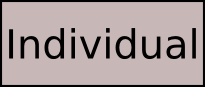
\includegraphics{./images/drobne/individual.png}}
 % class.png: 194x86 pixel, 90dpi, 5.48x2.43 cm, bb=0 0 155 69
 \\ \hline

PW005: & Property &
 \scalebox{0.30}{
\includegraphics{./images/drobne/property.png}}
 % class.png: 194x86 pixel, 90dpi, 5.48x2.43 cm, bb=0 0 155 69
 \\ \hline

PW006: & Datatype &
 \scalebox{0.30}{
\includegraphics{./images/drobne/datatype.png}}
 % class.png: 194x86 pixel, 90dpi, 5.48x2.43 cm, bb=0 0 155 69
 \\ \hline

PW007: & Anonymous Class &
 \scalebox{0.30}{
\includegraphics{./images/drobne/anonymousClass.png}}
 % class.png: 194x86 pixel, 90dpi, 5.48x2.43 cm, bb=0 0 155 69
 \\ \hline

PW008: & Subclass &
 \scalebox{0.30}{
\includegraphics{./images/drobne/subclass.png}}
 % class.png: 194x86 pixel, 90dpi, 5.48x2.43 cm, bb=0 0 155 69
 \\ \hline

PW009: & instanceOf &
 \scalebox{0.30}{
\includegraphics{./images/drobne/instanceOf.png}} \newline
 \scalebox{0.30}{
\includegraphics{./images/drobne/instanceOfDatatype.png}}
 % class.png: 194x86 pixel, 90dpi, 5.48x2.43 cm, bb=0 0 155 69
 \\ \hline

PW010: & equivalentClass &
 \scalebox{0.30}{
\includegraphics{./images/drobne/equivalentClass.png}}
 % class.png: 194x86 pixel, 90dpi, 5.48x2.43 cm, bb=0 0 155 69
 \\ \hline

PW011: & disjointWith &
 \scalebox{0.30}{
\includegraphics{./images/drobne/disjointWith.png}}
 % class.png: 194x86 pixel, 90dpi, 5.48x2.43 cm, bb=0 0 155 69
 \\ \hline

PW012: & differentFrom / allDifferent &
 \scalebox{0.30}{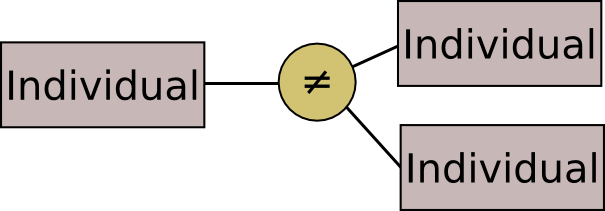
\includegraphics{./images/drobne/allDifferent.png}}
 % class.png: 194x86 pixel, 90dpi, 5.48x2.43 cm, bb=0 0 155 69
 \\ \hline

PW013: & sameAs &
 \scalebox{0.30}{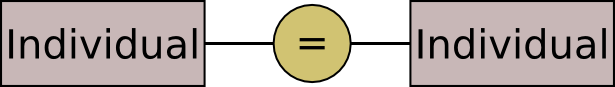
\includegraphics{./images/drobne/sameAs.png}}
 % class.png: 194x86 pixel, 90dpi, 5.48x2.43 cm, bb=0 0 155 69
 \\ \hline

PW014: & oneOf &
 \scalebox{0.30}{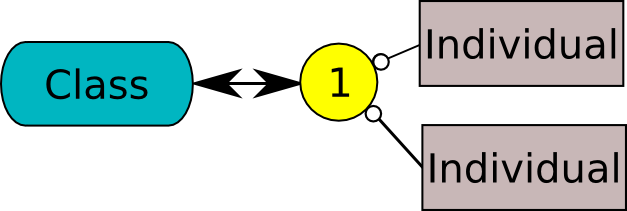
\includegraphics{./images/drobne/oneOf.png}}
 % class.png: 194x86 pixel, 90dpi, 5.48x2.43 cm, bb=0 0 155 69
 \\ \hline

PW015: & unionOf &
 \scalebox{0.30}{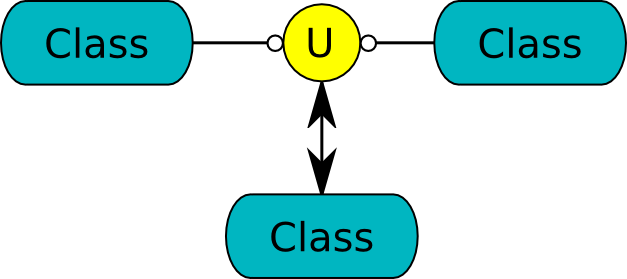
\includegraphics{./images/drobne/unionOf.png}}
 % class.png: 194x86 pixel, 90dpi, 5.48x2.43 cm, bb=0 0 155 69
 \\ \hline

PW016: & intersectionOf &
 \scalebox{0.30}{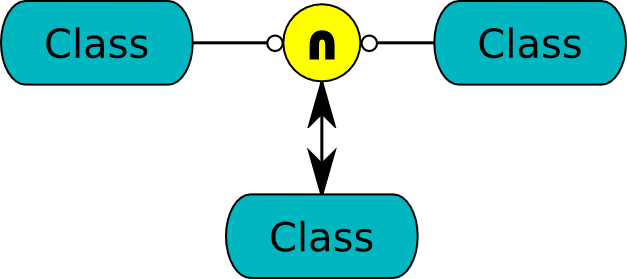
\includegraphics{./images/drobne/intersectionOf.png}}
 % class.png: 194x86 pixel, 90dpi, 5.48x2.43 cm, bb=0 0 155 69
 \\ \hline

PW017: & complementOf &
 \scalebox{0.30}{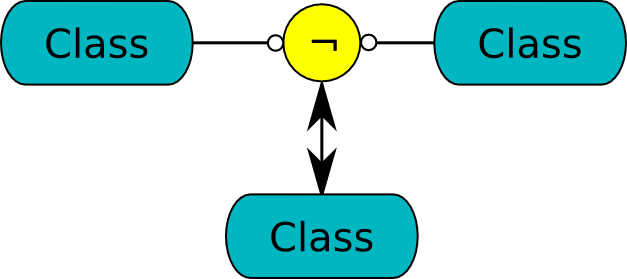
\includegraphics{./images/drobne/complementOf.png}}
 % class.png: 194x86 pixel, 90dpi, 5.48x2.43 cm, bb=0 0 155 69
 \\ \hline

PW018: & subProperty &
 \scalebox{0.30}{
\includegraphics{./images/drobne/subProperty.png}}
 % class.png: 194x86 pixel, 90dpi, 5.48x2.43 cm, bb=0 0 155 69
 \\ \hline

PW019: & inverseOf (property) &
 \scalebox{0.30}{
\includegraphics{./images/drobne/inverseOf.png}} \newline
\scalebox{0.30}{
\includegraphics{./images/drobne/inverseOfProperty.png}}
 % class.png: 194x86 pixel, 90dpi, 5.48x2.43 cm, bb=0 0 155 69
 \\ \hline

PW020: & equivalentProperty &
 \scalebox{0.30}{
\includegraphics{./images/drobne/equivalentProperty.png}}
 % class.png: 194x86 pixel, 90dpi, 5.48x2.43 cm, bb=0 0 155 69
 \\ \hline

PW021: & functionalProperty &
 \scalebox{0.30}{
\includegraphics{./images/drobne/functionalProperty.png}}
 % class.png: 194x86 pixel, 90dpi, 5.48x2.43 cm, bb=0 0 155 69
 \\ \hline

PW022: & inverseFunctionalProperty &
 \scalebox{0.30}{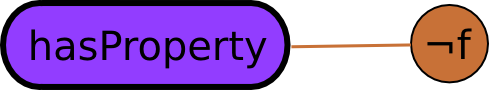
\includegraphics{./images/drobne/inverseFunctionalProperty.png}}
 % class.png: 194x86 pixel, 90dpi, 5.48x2.43 cm, bb=0 0 155 69
 \\ \hline

PW023: & symmetricProperty &
 \scalebox{0.30}{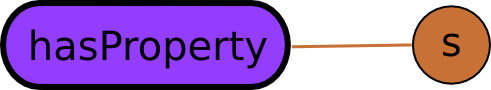
\includegraphics{./images/drobne/symmetricProperty.png}}
 % class.png: 194x86 pixel, 90dpi, 5.48x2.43 cm, bb=0 0 155 69
 \\ \hline

PW024: & transitiveProperty &
 \scalebox{0.30}{
\includegraphics{./images/drobne/transitiveProperty.png}}
 % class.png: 194x86 pixel, 90dpi, 5.48x2.43 cm, bb=0 0 155 69
 \\ \hline

PW025: & hasProperty &
 \scalebox{0.25}{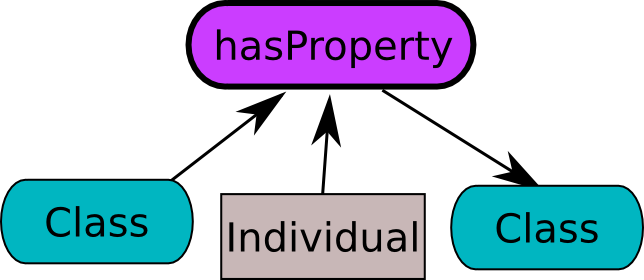
\includegraphics{./images/drobne/hasProperty.png}}
 % class.png: 194x86 pixel, 90dpi, 5.48x2.43 cm, bb=0 0 155 69
 \\ \hline

PW026: & domain &
 \scalebox{0.25}{
\includegraphics{./images/drobne/domain.png}}
 % class.png: 194x86 pixel, 90dpi, 5.48x2.43 cm, bb=0 0 155 69
 \\ \hline

PW027: & range &
 \scalebox{0.25}{
\includegraphics{./images/drobne/range.png}}
 % class.png: 194x86 pixel, 90dpi, 5.48x2.43 cm, bb=0 0 155 69
 \\ \hline

PW028: & allValuesFrom &
 \scalebox{0.25}{
\includegraphics{./images/drobne/allValuesFrom.png}}
 % class.png: 194x86 pixel, 90dpi, 5.48x2.43 cm, bb=0 0 155 69
 \\ \hline

PW029: & someValuesFrom &
 \scalebox{0.25}{
\includegraphics{./images/drobne/someValuesFrom.png}}
 % class.png: 194x86 pixel, 90dpi, 5.48x2.43 cm, bb=0 0 155 69
 \\ \hline

PW030: & minCardinality / maxCardinality &
 \scalebox{0.30}{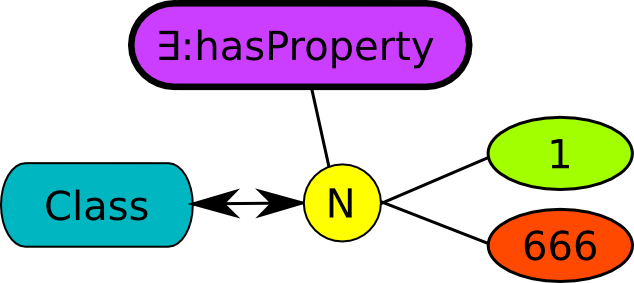
\includegraphics{./images/drobne/cardinalityminmax.png}}
 % class.png: 194x86 pixel, 90dpi, 5.48x2.43 cm, bb=0 0 155 69
 \\ \hline

PW031: & cardinality &
 \scalebox{0.30}{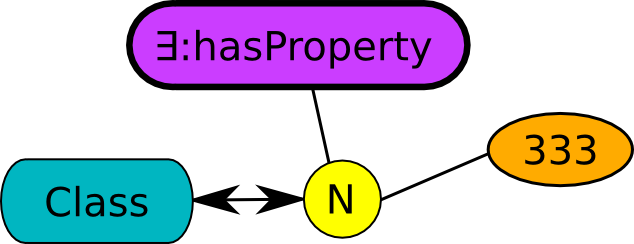
\includegraphics{./images/drobne/cardinality.png}}
 % class.png: 194x86 pixel, 90dpi, 5.48x2.43 cm, bb=0 0 155 69
 \\ \hline


\end{longtable}
% \end{table}